\documentclass[11pt, a4paper, twoside]{article}   	% use "amsart" instead of "article" for AMSLaTeX format

\usepackage{geometry}                		% See geometry.pdf to learn the layout options. There are lots.
\usepackage{pdfpages}
\usepackage{caption}
\usepackage{minted}
\usepackage[german]{babel}			% this end the next are needed for german umlaute
\usepackage[utf8]{inputenc}
\usepackage{color}
\usepackage{graphicx}
\usepackage{titlesec}
\usepackage{fancyhdr}
\usepackage{lastpage}
\usepackage{hyperref}
\usepackage[autostyle=false, style=english]{csquotes}
\usepackage{mathtools}
\usepackage{tabularx}
% http://www.artofproblemsolving.com/wiki/index.php/LaTeX:Symbols#Operators
% =============================================
% Layout & Colors
% =============================================
\geometry{
   a4paper,
   total={210mm,297mm},
   left=20mm,
   right=20mm,
   top=20mm,
   bottom=30mm
 }	

\definecolor{myred}{rgb}{0.8,0,0}
\definecolor{mygreen}{rgb}{0,0.6,0}
\definecolor{mygray}{rgb}{0.5,0.5,0.5}
\definecolor{mymauve}{rgb}{0.58,0,0.82}

\setcounter{secnumdepth}{4}


% the default java directory structure and the main packages
\newcommand{\srcDir}{../source/Grammar/}
% =============================================
% Code Settings
% =============================================
\newenvironment{code}{\captionsetup{type=listing}}{}
\newmintedfile[cppSourceFile]{cpp}{
	linenos=true, 
	frame=single, 
	breaklines=true, 
	tabsize=2,
	numbersep=5pt,
	xleftmargin=10pt,
	baselinestretch=1,
	fontsize=\footnotesize
}
\newmintinline[inlineCpp]{cpp}{}
\newminted[cppSource]{cpp}{
	breaklines=true, 
	tabsize=2,
	autogobble=true,
	breakautoindent=false
}
% =============================================
% Page Style, Footers & Headers, Title
% =============================================
\title{Übung 1}
\author{Thomas Herzog}

\lhead{Übung 1}
\chead{}
\rhead{
\includegraphics[scale=0.10]{FHO_Logo_Students.jpg}}

\lfoot{S1610454013}
\cfoot{}
\rfoot{ \thepage / \pageref{LastPage} }
\renewcommand{\footrulewidth}{0.4pt}
% =============================================
% D O C U M E N T     C O N T E N T
% =============================================
% =============================================
% 2016.10.13: 1 
% 2016.10.14: 2
% =============================================

\pagestyle{fancy}
\begin{document}
\setlength{\headheight}{15mm}
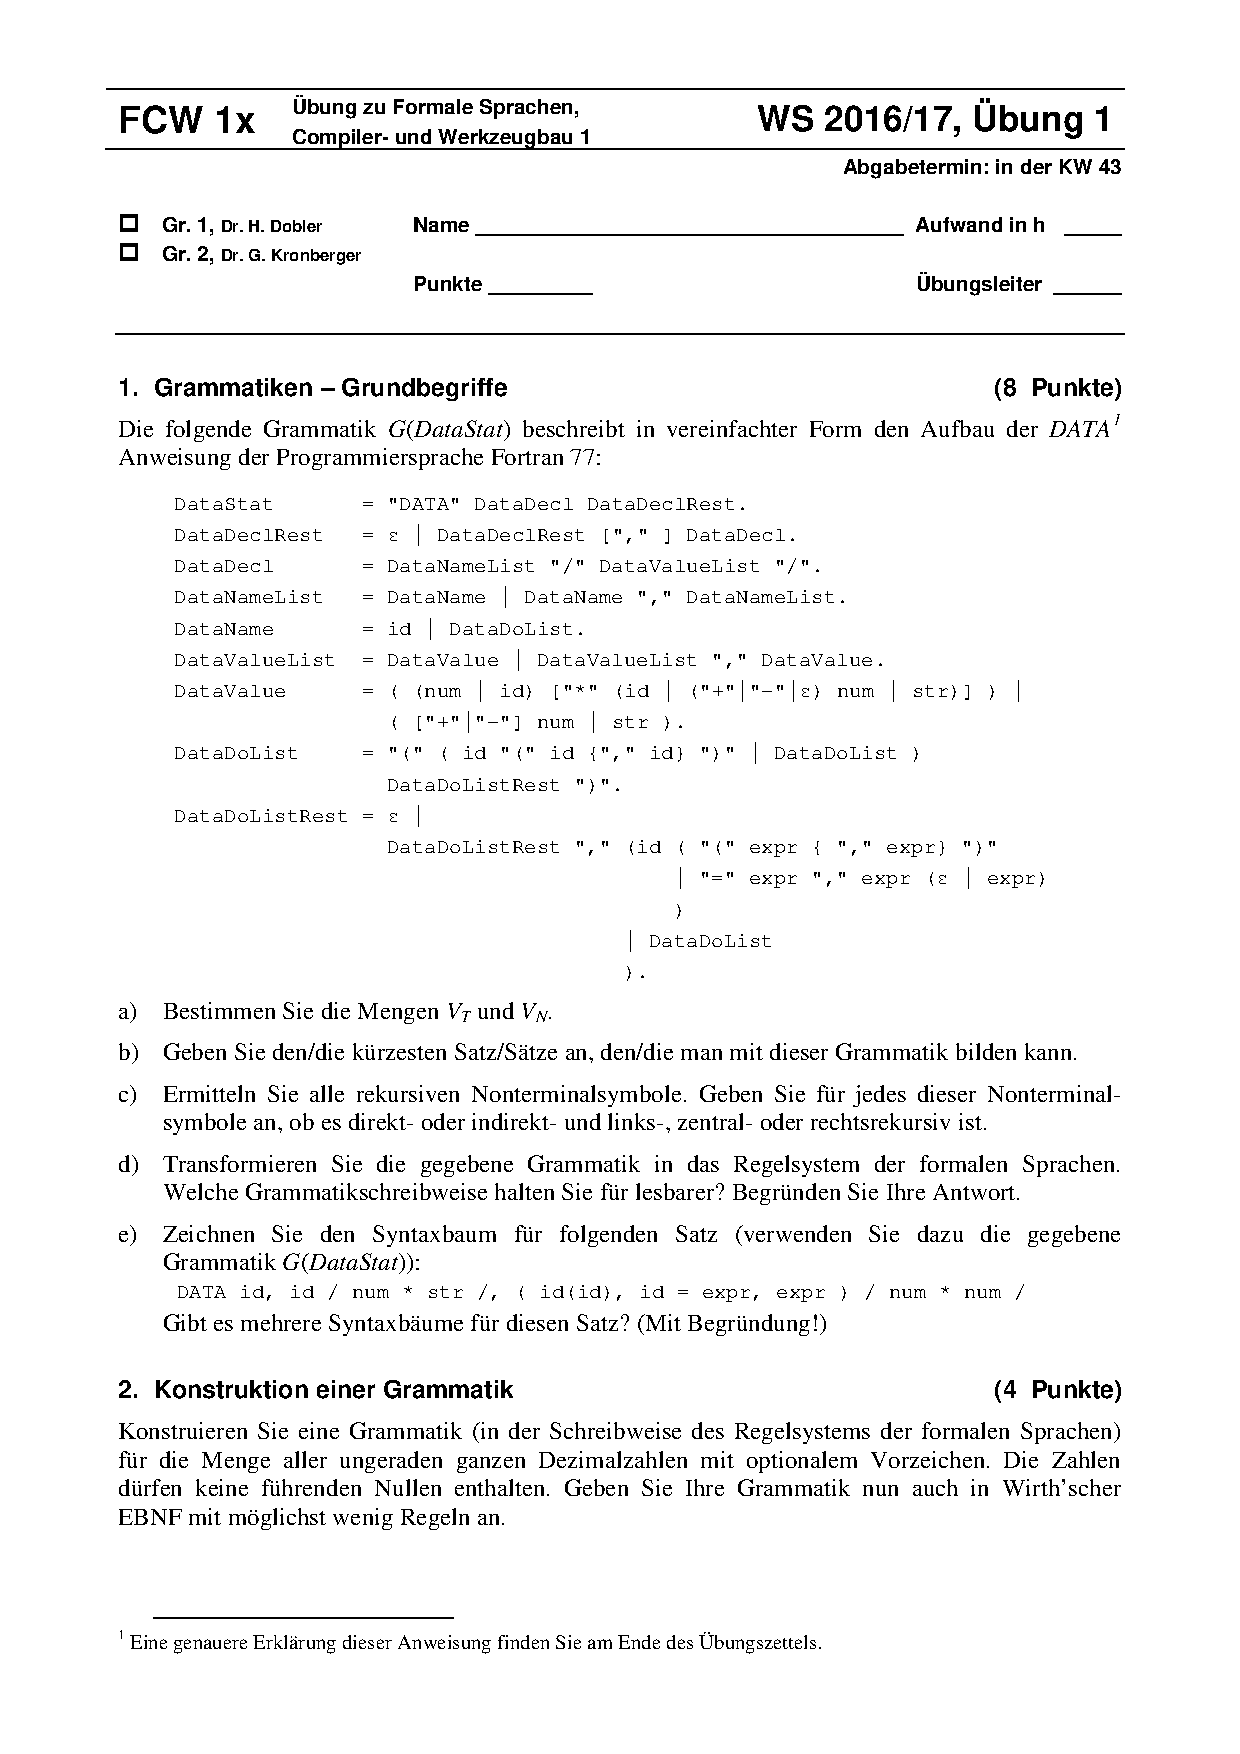
\includepdf[pages={1,2}]{Fcw1x01A.pdf}

% Section gramar and basics 
\section {Grammatiken - Grundbegriffe}
\label{sec:grammar-basics}
Dieser Abschnitt behandelt die Aufgabe 1 der ersten Übung.
\subsection{Die Mengen $V_{T}$ und $V_{N}$}
$V_{N}=\{$ DataStat, DataDeclRest, DataDecl, DataNameList, DataName, DataValueList, DataValue, DataDoList, DataDoListRest $\}$
\newline
\newline
Alle Nichtterminalsymbole befinden sich links in der Grammatik, wobei das Nichtterminalsymbol \emph{DataStat} das Satzsymbol ist.
\newline
\newline
\newline
$V_{T}=\{$ \enquote{DATA},\enquote{,}, \enquote{/}, \enquote{(}, \enquote{)},\enquote{=}, \enquote{*}, \enquote{+}, \enquote{-}, \enquote{=}, expr, id, num, str $\}$
\newline
\newline
Alle Terminalsymbole kommen nicht auf der linken Seite der Grammatik vor und können nicht weiter abgeleitet werden. Das Symbol \enquote{$\epsilon$} ist ein Metasymbol, das die leere Kette repräsentiert und ist weder ein Nichtterminalsymbol noch ein Terminalsymbol.
\newline
\newline
\newline
$V=V_{T} \cup V_{N}$
\newline
\newline
Die Menge $V$ ist das Alphabet der Grammatik und ist die Vereinigung der Menge der Nichtterminalsymbole und der Menge der Terminalsymbole. Da das Symbol $\epsilon$ ein Metasymbol ist, ist es nicht Teil der Grammatik und auch kein Teil des Alphabets der Grammatik.

\subsection{Kürzeste Sätze der Grammatik}
DataStat $\xRightarrow{L}$ \enquote{DATA} \underline{DataDecl} DataDeclRest
\newline
\null\hspace{1.55cm} $\xRightarrow{L}$ \enquote{DATA} \underline{DataNameList} \enquote{/} DataValueList \enquote{/} DataDeclRest
\newline
\null\hspace{1.55cm} $\xRightarrow{L}$ \enquote{DATA} \underline{DataName} \enquote{/} DataValueList \enquote{/} DataDeclRest
\newline
\null\hspace{1.55cm} $\xRightarrow{L}$ \enquote{DATA} id \enquote{/} \underline{DataValueList} \enquote{/} DataDeclRest
\newline
\null\hspace{1.55cm} $\xRightarrow{L}$ \enquote{DATA} id \enquote{/} \underline{DataValue} \enquote{/} DataDeclRest
\newline
\null\hspace{1.55cm} $\xRightarrow{L}$ \enquote{DATA} id \enquote{/} num  \enquote{/} \underline{DataDeclRest}
\newline
\null\hspace{1.55cm} $\xRightarrow{L}$ \enquote{DATA} id \enquote{/} num  \enquote{/}
\newline
\newline
\newline
%
DataStat $\xRightarrow{L}$ \enquote{DATA} \underline{DataDecl} DataDeclRest
\newline
\null\hspace{1.55cm} $\xRightarrow{L}$ \enquote{DATA} \underline{DataNameList} \enquote{/} DataValueList \enquote{/} DataDeclRest
\newline
\null\hspace{1.55cm} $\xRightarrow{L}$ \enquote{DATA} \underline{DataName} \enquote{/} DataValueList \enquote{/} DataDeclRest
\newline
\null\hspace{1.55cm} $\xRightarrow{L}$ \enquote{DATA} id \enquote{/} \underline{DataValueList} \enquote{/} DataDeclRest
\newline
\null\hspace{1.55cm} $\xRightarrow{L}$ \enquote{DATA} id \enquote{/} \underline{DataValue} \enquote{/} DataDeclRest
\newline
\null\hspace{1.55cm} $\xRightarrow{L}$ \enquote{DATA} id \enquote{/} id  \enquote{/} \underline{DataDeclRest}
\newline
\null\hspace{1.55cm} $\xRightarrow{L}$ \enquote{DATA} id \enquote{/} id  \enquote{/}
\newpage

\parindent0pt DataStat $\xRightarrow{L}$ \enquote{DATA} \underline{DataDecl} DataDeclRest
\newline
\null\hspace{1.55cm} $\xRightarrow{L}$ \enquote{DATA} \underline{DataNameList} \enquote{/} DataValueList \enquote{/} DataDeclRest
\newline
\null\hspace{1.55cm} $\xRightarrow{L}$ \enquote{DATA} \underline{DataName} \enquote{/} DataValueList \enquote{/} DataDeclRest
\newline
\null\hspace{1.55cm} $\xRightarrow{L}$ \enquote{DATA} id \enquote{/} \underline{DataValueList} \enquote{/} DataDeclRest
\newline
\null\hspace{1.55cm} $\xRightarrow{L}$ \enquote{DATA} id \enquote{/} \underline{DataValue} \enquote{/} DataDeclRest
\newline
\null\hspace{1.55cm} $\xRightarrow{L}$ \enquote{DATA} id \enquote{/} str  \enquote{/} \underline{DataDeclRest}
\newline
\null\hspace{1.55cm} $\xRightarrow{L}$ \enquote{DATA} id \enquote{/} str  \enquote{/}
\newline
\newline
Das Nichtterminalsymbol \emph{DataValue} kann in drei Varianten abgeleitet werden, \emph{id}, \emph{num} und \emph{str}. Die Satzlänge bleibt bei jeder der drei Ableitungen des Nichtterminalsymbols \emph{DataValue} gleich.

\subsection{Rekursionen der Nichtterminalsymbole}
    \begin{tabularx}{\textwidth}{|>{\centering}X|>{\centering}X|>{\centering\arraybackslash}X|}
    \hline
    \textbf{Nichtterminalsymbol} & \textbf{direkt/indirekt rek.} & \textbf{links/rechts rek.} \\ \hline
    DataDeclRest                 &           direkt rek.         &           links rek.\\ \hline
    DataDecl                     &               -               &             -           
    \\ \hline
    DataNameList                 &           direkt rek.         &           rechts rek. \\ \hline
    DataName                     &               -               &             -    
    \\ \hline
    DataValueList                &           direkt rek.         &           links rek. \\ \hline
    DataValue                    &               -               &             -    
    \\ \hline
    DataDoList                   &           direkt rek.         &           zentral rek.\\ \hline
    DataDoList                   &           indirekt rek.       &           zentral rek.\\ \hline
    DataDoListRest               &           indirekt rek.       &           zentral rek.\\ \hline
    \end{tabularx}
\newline
\newline
Die beiden indirekten Rekursionen der Nichtterminalsymbole \emph{DataDoList} und \emph{DataDoListRest} ergeben sich aus der Tatsache, dass wenn es eine indirekte Rekursion gibt, es auch eine zweite Rekursion geben muss. Ich gehe davon aus, dass ich alle Rekursionen gefunden habe, wobei angemerkt sei, dass es sehr schwer ist Rekursionen aus einer Grammatik auszulesen. 

\subsection{Transformation in das Regelsystem der formalen Sprachen}
\begin{tabularx}{\textwidth}{p{80pt} @{$\rightarrow$ \hspace{10pt}} X}
	DataStat      & DATA DataDecl DataDeclRest \\
	DataDeclRest  &  $\epsilon$ $|$  DataDeclRest , DataDecl $|$ DataDeclRest   DataDecl  \\
	DataDecl       & DataNameList / DataValueList /\\
	DataNameList   & DataName $|$ DataName , DataNameList\\
	DataName       & id $|$ DataDoList\\
	DataValueList  & DataValue $|$ DataValueList , DataValue\\
	DataValue      & num DerefValue $|$ id DerefValue $|$ NumOrStr\\
	NumValue       & num $|$ + num $|$ - num\\
	NumOrStr       & NumValue $|$ str\\
	DerefValue     & $\epsilon$ $|$ * id $|$ * NumOrStr\\
	DataDoList     & ( IdList DataDoListRest ) $|$ ( DataDoList DataDoListRest )\\
	CommaId        & $\epsilon$ $|$ , id CommaId\\
    IdList         & id ( id CommaId )	\\
    DataDoListRest & $\epsilon$ $|$ DataDoListRest , DoListRestOpt \\
    ComaExpr       & $\epsilon$ $|$ , expr CommaExpr\\
    ExprList       & ( expr CommaExpr )\\
    OptExpr        & $\epsilon$ $|$ expr\\
    EqualExpr      & = expr , expr OptExpr\\
    DoListRestOpt & id ExprList $|$ id EuqlExpr $|$ DataDoList
\end{tabularx}
\newpage
Um diesen Punkt der Aufgabe \ref{sec:grammar-basics} zu lösen wurden die Optionen und Schleifen von innen nach außen aufgelöst und in eigene Nichtterminalsybole ausgelagert. Das ist notwendig, da das Regelwerk der formalen Sprachen diese Konstrukte nicht kennt und die Konstrukte Optionen und Schleifen in \emph{Oder} Konstrukte umgewandelt werden müssen. Bsp.: [num, str] $\equiv$ $\epsilon$ $|$ num $|$ str
\newline
\newline
Ich halte die Schreibweise der Wirth'schen EBNF für lesbarer, da in dieser Schreibweise mehr Konstrukte wie Optionen und Schleifen zur Verfügung stehen und dadurch die Grammatik durch weniger Regeln definiert werden kann, was die Grammatik übersichtlicher macht.
\newpage
\subsection{Syntaxbaum}
Die Abbildung \ref{fig:syntaxtree} zeigt den Syntaxbaum des Satzes
\newline
\emph{DATA id, id / num * str /, ( id(id), id = expr, expr ) / num * num /}.
\begin{figure}[h]
\centering
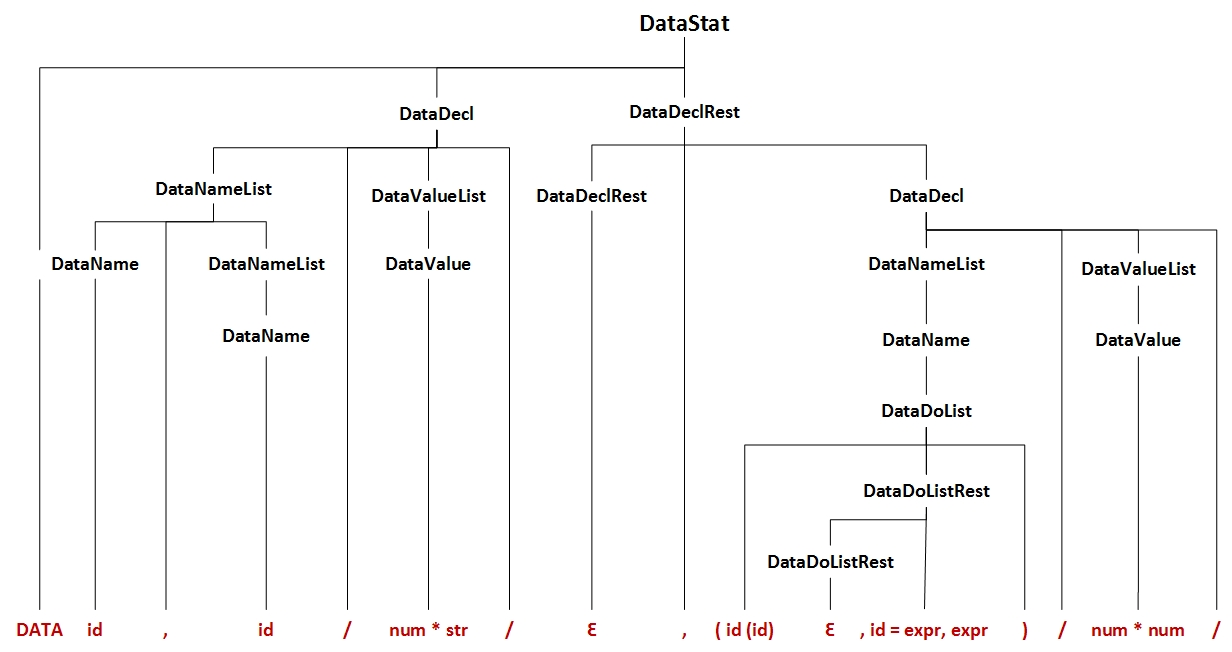
\includegraphics[scale=0.70,angle=90]{Syntaxtree.jpg}
\caption{Syntaxbaum}
\label{fig:syntaxtree}
\end{figure}
\ \newline
Es gibt für den gegebenen Satz nur einen Syntaxbaum, da es keine Möglichkeit gibt, den Satz mit der gegebenen Grammatik über andere Wege in einen anderen Syntaxbaum zu überführen. Das bedeutet aber nicht dass die Grammatik eindeutig ist, da es nötig wäre alle möglichen Sätze in alle ihre möglichen Syntaxbäume zu überführen, was mit der gegebenen Grammatik nicht möglich ist, da mit der gegebenen Grammatik unendliche viele Sätze erstellt werden können.
\newpage

\section{Konstruktion einer Grammatik}
Dieser Abschnitt behandelt die Aufgabe 2 der ersten Übung.
\subsection{Mit dem Regelsystem der formalen Sprachen}
In diesem Abschnitt wird die Grammatik mit dem Regelsystem der formalen Sprachen angeführt.
\newline
\newline
\begin{tabularx}{\textwidth}{p{100pt} @{$\rightarrow$ \hspace{10pt}} X}
	SignedOddDecimal  & Sign IntegerNoZero AllIntegerOpt, AllIntegerOpt OddInteger\\
	Sign              & $\epsilon$ $|$ + $|$ -\\
	OddInteger        & 1 $|$ 3 $|$ 5 $|$ 7 $|$ 9\\ 
	IntegerNoZero     & 2 $|$ 4 $|$ 6 $|$ 8 $|$ OddInteger\\
	AllInteger        & 0 $|$ IntegerNoZero\\
	AllIntegerOpt     & $\epsilon$ $|$ AllInteger $|$ AllIntegerOpt\\
\end{tabularx}

\subsection{Mit der Wirth'schen EBNF}
Dieser Abschnitt wird die Grammatik mit der With'schen EBNF angeführt.
\newline
\newline
\begin{tabularx}{\textwidth}{p{100pt} @{= \hspace{10pt}} X}
	SignedOddDecimal  & [+ $|$ -] IntegerNoZero \{0 $|$ IntegerNoZero\}, \{0 $|$ IntegerNoZero\} OddInteger\\
	OddInteger        & 1 $|$ 3 $|$ 5 $|$ 7 $|$ 9\\ 
	IntegerNoZero     & 2 $|$ 4 $|$ 6 $|$ 8 $|$ OddInteger\\	
\end{tabularx}
\newline
\newline

% Section Oo-implementation of an grammar
\section {Oo-Implementierung von Grammatiken}
\label{sec:oo-grammar-impl}
Dieser Abschnitt behandelt die Aufgabe 3 der ersten Übung.
\subsection{\emph{Grammar *epsilonFreeGrammarOf(Grammar *grammar)}}
\label{sec:epsilon-free-grammar-subsc}
Die Implementierung erfolgte in den Quelltextdateien \emph{GrammarUtil.hpp} und \emph{GrammarUtil.cpp} und wurde im Namensraum \emph{GrammarUtil} organisiert.
\subsubsection{Quelltexte}
\begin{code}
	\caption{GrammarUtil.hpp}
	\cppSourceFile{\srcDir/GrammarUtil.hpp}
\end{code}
\begin{code}
	\caption{GrammarUtil.cpp}
	\label{source:grammar-util}
	\cppSourceFile{\srcDir/GrammarUtil.cpp}
\end{code}
\ \newpage

\subsubsection{Tests}
Dieser Abschnitt behandelt die Tests der Implementierung aus dem Abschnitt \ref{sec:epsilon-free-grammar-subsc}.
\begin{figure}[h]
\centering
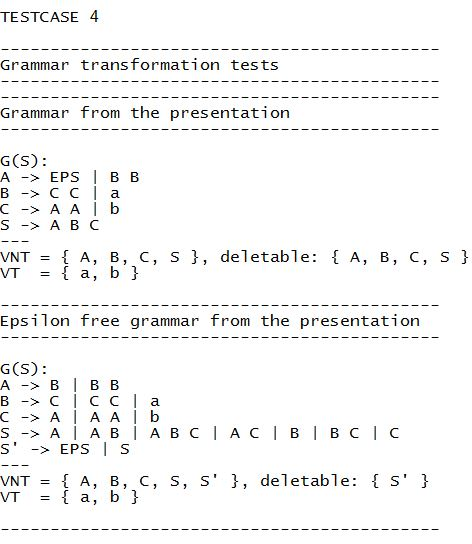
\includegraphics[scale=0.80]{tests_epsilon_free_1.JPG}
\caption{Epsilonfreie Grammatik der vorgegebenen Grammatik}
\label{fig:hands-on-material-epsilon-free}
\end{figure}
\ \newline
Die Tests aus Abbildung \ref{fig:hands-on-material-epsilon-free} zeigen die vorgegebenen Grammatik aus den Vorlesungsunterlagen und die epsilonfreie Variante dieser Grammatik. 

\ \newpage
\begin{figure}[h]
\centering
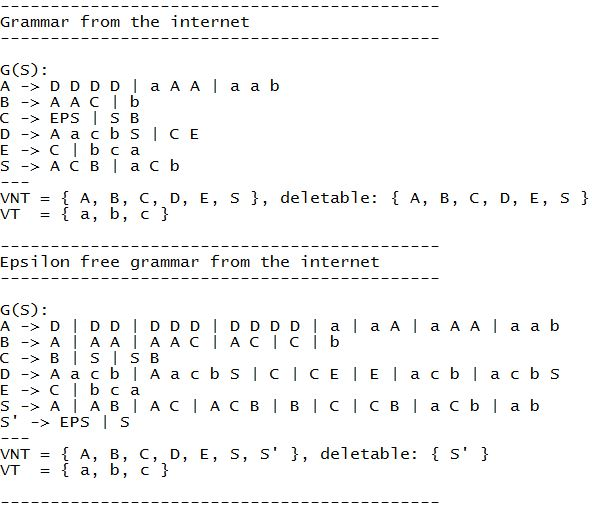
\includegraphics[scale=0.80]{tests_epsilon_free_2.JPG}
\caption{Epsilonfreie Grammatik des Internetbeispiels}
\label{fig:internet-epsilon-free}
\end{figure}
\ \newline
Die Tests aus Abbildung \ref{fig:internet-epsilon-free} zeigen eine Grammatik, die im Internet unter folgender \emph{URL} \url{http://www.informatikseite.de/theorie/node43.php} gefunden werden kann und die epsilonfreie Variante dieser Grammatik. 
\newpage

\subsection{\emph{Language *generateLanguage(Grammar *g, int maxLen)}}
\label{sec:generate-language-subsec}
Alle möglichen Sätze der Sprache bis zur maximal erlaubten Länge, die durch die vorgegebene Grammatik möglich sind, werden in der Funktion \inlineCpp{derive(const Grammar *_grammar, int maxLength)} durch das Ermitteln aller möglichen Ableitungen bis zur erlaubten Satzlänge der Grammatik ermittelt.
\newline
\newline
Die Sätze der Sprache bestehen aus Wiederholungen von \emph{ab}, \emph{ba} und Folgen von nur \emph{a} oder nur \emph{b}. Die Wiederholungen von \emph{ab} und \emph{ba} lassen sich schon aus der Grammatik aus den beiden Sequenzen \emph{bS} und \emph{aS} auslesen. 

\subsubsection{Quelltexte}
In diesem Abschnitt werden die Quelltextdateien der Implementierung angeführt. Die Implementierung erfolgte in den Quelltextdateien \emph{LanguageUtil.hpp}, \emph{LanguageUtil.cpp}, \emph{Language.hpp} und \emph{Language.hpp}.
\begin{code}
	\caption{Language.hpp}
	\cppSourceFile{\srcDir/Language.hpp}
\end{code}
\begin{code}
	\caption{Language.cpp}
	\label{source:language}
	\cppSourceFile{\srcDir/Language.cpp}
\end{code}
\begin{code}
	\caption{LanguageUtil.hpp}
	\cppSourceFile{\srcDir/LanguageUtil.hpp}
\end{code}
\begin{code}
	\caption{LanguageUtil.cpp}
	\cppSourceFile{\srcDir/LanguageUtil.cpp}
\end{code}

\subsubsection{Tests}
Dieser Abschnitt behandelt die Tests der Implementierung aus dem Abschnitt \ref{sec:generate-language-subsec}.
\begin{figure}[h]
\centering
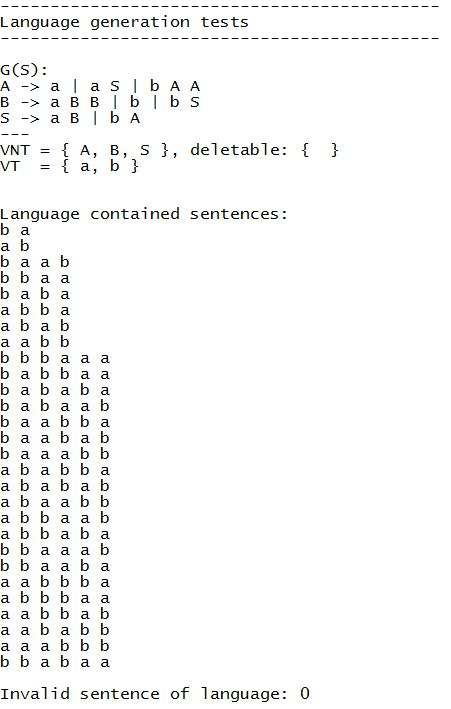
\includegraphics[scale=0.75]{tests_generate_language_1.JPG}
\caption{Tests der Generierung der Sprache}
\label{fig:generate-tests-language}
\end{figure}
\ \newline
Die Tests aus Abbildung \ref{fig:generate-tests-language} zeigen die generierte Sprache für die vorgegebene Grammatik. 
\newpage

\subsection{\emph{bool Language::hasSentence(Sequence *s) const}}
Dieser Abschnitt behandelt die Implementierung der Klassenmethode \emph{hasSentence} für die Klasse \emph{Language}, die überprüft ob ein gegebener Satz ein Satz dieser Sprache ist. Die Implementierung ermittelt rekursiv ob ein Satz über Reduktion zum Satzsymbol reduziert werden kann. Kann ein Satz bis zum Satzsymbol reduziert werden, dann ist dieser Satz auch ein Satz dieser Sprache. Da der implementierte Algorithmus alle möglichen Reduktionen durchprobiert verschlechtert sich das Laufzeitverhalten dieser Methode erheblich je länger die Sätze sind.

\subsubsection{Quelltexte}
Die Quelltexte der Implementierung sind bereits in den Quelltexten \ref{source:language}[Language.cpp] und \ref{source:grammar-util}[GrammarUtil.cpp] angeführt.

%\subsubsection{MainFX.java}
%Diese Klasse stellt die Main Klasse für die JavaFX Applikation dar.
%\begin{code}
%	\caption{MainFX.java}
%	\javaSourceFile{\fxSource/main/MainFX.java}
%\end{code}
\end{document}